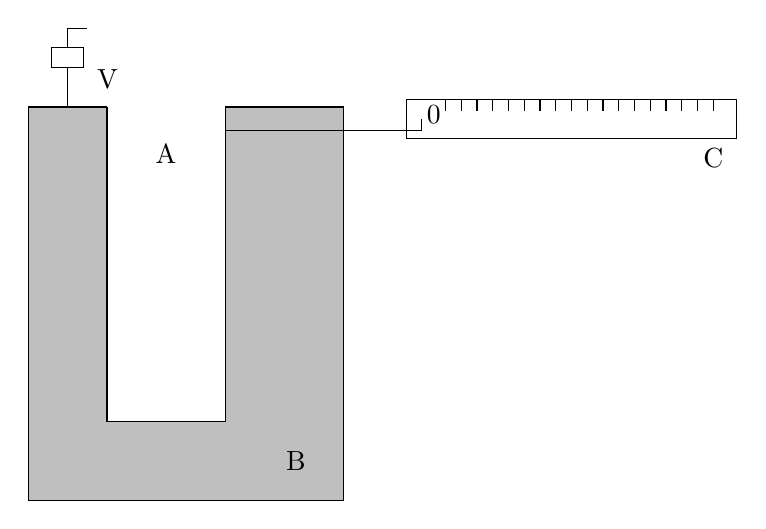
\begin{tikzpicture}[scale=1]
% container body (gray)
\fill[gray!50] (0,0) rectangle (4,5);
\draw (0,0) rectangle (4,5);
% inner white well (region A)
\fill[white] (1,1) rectangle (2.5,5.01);
\draw (1,5) -- (1,1) -- (2.5,1) -- (2.5,5);
% region labels
\node at (1.75,4.4) {A};
\node at (3.4,0.5) {B};
% valve V at top-left
\draw (0.5,5) -- (0.5,5.5);
\draw (0.3,5.5) rectangle (0.7,5.75);
\draw (0.5,5.75) -- (0.5,6.0) -- (0.75,6.0);
\node[right] at (0.75,5.35) {V};
% tube from well to ruler
\draw (2.5,4.7) -- (5,4.7) -- (5,4.85);
% ruler C
\draw (4.8,4.6) rectangle (9,5.1);
\node at (5.15,4.9) {0};
\foreach \x in {5.3,5.5,...,8.8} \draw (\x,5.1) -- (\x,4.95);
\node at (8.7,4.35) {C};
\end{tikzpicture}
